\chapter{Examples}

\section {Introduction}

We will present multiple examples to show how our tools can inspect the runtime behaiour of four applications: a trivial example application, emsim, cppcheck and bzip. We will also examine the overhead of our implementation compared to other tools built using Intel Pin and other dynamic instrumentation frameworks.

\section{Examples}

\subsection{Trivial example}

The example shown in \ref{cap4:test2} shows a trivial application that performs a variety of memory operations on a dynamically allocated array and some stack variables. Table \ref{cap4:test2references} shows these memory locations as they are detected by our tool.

\begin{figure}
	\begin{center}
		\inputminted[linenos, fontsize=\scriptsize]{c}{test2.c}
	\end{center}
	\caption{\texttt{test2.c}: Trivial example}
	\label{cap4:test2}
\end{figure}

\begin{figure}
	\begin{center}
		\begin{tabular}{l l l}
			Id & Size & Name \\
			31 & 350 & fe2010 \\
			32 & 8 & S: 7fff74714e28:-16:1 \\
			33 & 4 & S: 7fff74714e24:-20:1 \\
		\end{tabular}
	\end{center}
	\caption{\texttt{test2.c}: Trivial example references}
	\label{cap4:test2references}
\end{figure}

\subsection {Section Analysis -- emsim}

Section Analysis is most useful in applications that are not trivial to understand using source code inspection. To illustrate this we will use our tools to find parallelization opportunities in emsim \cite{emsim}, a simulator for the UEFA European Championship.

The file most relevant for the analysis is \texttt{emsim\_seq.c} and can be seen in Figure \ref{cap4:emsim:seq}. There are a number of loops in this file and a developer must determine which can be parallelize and what benefit it will provide. The \texttt{playEM} function uses complex pointer arithmetic making inspection very difficult. Without a thorough understanding of how emsim works it is impossible to determine whether loop iterations access the same memory locations.

First we will look at the loop on line 12. It repeatedly calls \texttt{playGroup}. We know that it takes up most of the execution time as can be seen in Figure \ref{cap4:emsim:profile}. Using Section analysis we will determine whether the loop iterations access the same memory locations.

\begin{figure}[!ht]
	\centering
	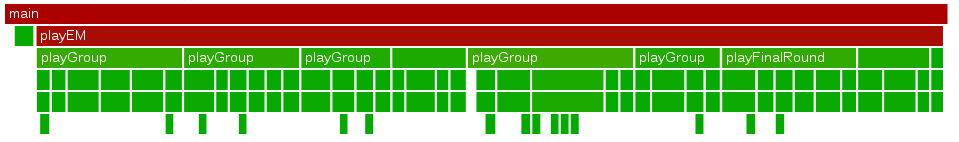
\includegraphics[width=1\textwidth]{profiling}
	\caption{Profile view of the execution the code using Parceive}
	\label{cap4:emsim:profile}
\end{figure}

\begin{figure}
	\begin{center}
		\inputminted[linenos, fontsize=\scriptsize]{c}{emsim_seq.c}
	\end{center}
	\caption{\texttt{emsim\_seq.c}: EM Simulator sequential implementation}
	\label{cap4:emsim:seq}
\end{figure}

\subsubsection*{Static analysis and Tagging}



\subsubsection*{Dynamic analysis}

\subsubsection*{Eliminating known conflicts}

\subsection {Pipeline Analysis -- pipeline}

\section{Performance}

In this Section we will compare the performance of our tool with an Intel Pin tool that performs no analysis, Parceive and memcheck (part of valgrind). We will test the applications presented in the previous sections.

\subsection{Intel Pin overhead}

\begin{figure}
	\begin{center}
		\inputminted[linenos, fontsize=\scriptsize]{c++}{../pintool/pintest.cpp}
	\end{center}
	\caption{\texttt{pintest.cpp}}
	\label{cap4:pintest}
\end{figure}

To determine the overhead of running an application using Intel Pin we have developed a trivial tool that performs no analysis and can be seen in Figure \ref{cap4:pintest}. For this test Intel Pin has been configured use its JIT compiles that is used both in our tools and in Parceive.

\begin{figure}
	\begin{center}
		\inputminted[linenos, fontsize=\scriptsize]{c++}{../pintool/pintestprobe.cpp}
	\end{center}
	\caption{\texttt{pintestprobe.cpp}}
	\label{cap4:pintestprobe}
\end{figure}

Pin is also able to execute applications without a JIT compiler, in probe mode \cite{pindoc}. This reduces its overhead considerably and we have created another trivial tool to illustrate this. It can be seen in Figure \ref{cap4:pintestprobe}. Unfortunately both our trivial tool and the examples provided for probe mode crash when executed in the environment described in Appendix \ref{appendix:setup}.

\subsection{Commands used}

Normal execution
\begin{lstlisting}[style=BashInputStyle]
<application>
\end{lstlisting}

Pin JIT
\begin{lstlisting}[style=BashInputStyle]
pin.sh -ifeellucky -t libpintool_pintest.so -- <application>
\end{lstlisting}

Pin Probe
\begin{lstlisting}[style=BashInputStyle]
pin.sh -ifeellucky -t libpintool_pintestprobe.so -- <application>
\end{lstlisting}

Parceive
\begin{lstlisting}[style=BashInputStyle]
pin.sh -ifeellucky -t parceive.so -- <application>
\end{lstlisting}

Valgrind
\begin{lstlisting}[style=BashInputStyle]
valgrind <application>
\end{lstlisting}

\texttt{pintool\_static.so}
\begin{lstlisting}[style=BashInputStyle]
pin.sh -ifeellucky -t libpintool_static.so
	-db test.db -- <application>
\end{lstlisting}

\texttt{pintool\_dynamic.so}
\begin{lstlisting}[style=BashInputStyle]
pin.sh -ifeellucky -t libpintool_static.so
	-db test.db -- <application>
\end{lstlisting}

\subsection{Filters and tags}

Filtering for our tools and Parceive has been enabled and is identical. System libraries and headers as well as sqlite have been excluded from analysis. Our tools have no tags configured, but will track all memory accesses by default similarly to Parceive. The exact filters and source.yaml can be seen in Figure \ref{cap4:compconfig}.

\begin{figure}
	\begin{center}
		\textbf{filter.yaml}
		\inputminted[linenos, fontsize=\scriptsize]{yaml}{../tests/filter.yaml}
				
		\textbf{source.yaml}
		\inputminted[linenos, fontsize=\scriptsize]{yaml}{../tests/emptysource.yaml}
		
		\textbf{blacklist.xml}
		\inputminted[linenos, fontsize=\scriptsize]{xml}{blacklist.xml}
		
		\textbf{filter.xml}
		\inputminted[linenos, fontsize=\scriptsize]{xml}{filter.xml}
	\end{center}
	\caption{Filters and tags used for comparison}
	\label{cap4:compconfig}
\end{figure}

\subsection{Disk cache}

Before executing each test the disk cache is dropped.

\subsection{Results}

\begin{tabular}{l|l|l|l}
	& Trivial example & emsim & pipeline \\ 
	\hline 
	Normal execution & 0m0.168s & 0m4.639s & 0m9.365s \\ 
	\hline 
	Pin JIT & 0m0.298s & 0m20.598s & 0m21.513s \\ 
	\hline 
	Pin probe mode & ? & ? & ? \\ 		
	\hline 
	Parceive & 0m15.273s & 1m26.135s & 5m51.329s \\ 
	\hline 
	Memcheck & 0m0.262s & 1m58.874s & 1m30.530s \\ 
	\hline 
	\texttt{pintool\_static.so} &  & &  \\ 
	\hline
	\texttt{pintool\_dynamic.so} &  & &  \\
	\hline
	\texttt{pintool\_static.so} No memory &  & &  \\ 
	\hline
	\texttt{pintool\_dynamic.so} No memory &  & &  \\
\end{tabular} 